% !TEX encoding = UTF-8
% !TEX TS-program = pdflatex
% !TEX root = ../Tesi.tex
% !TEX spellcheck = it-IT

%************************************************
\chapter{Realizzazione}
\label{cap:realizzazione}

Il progetto è stato realizzato attraverso la divisione in sotto problemi. Questo permette la sostituzione di una componente con un'altra in modo rapido ed sicuro in quanto viene a essere modificata solo la parte del codice interessata dall'operazione e non tutte le altre componenti, che rimangono invariate. Questo permette di testare singolarmente le parti senza necessità di avere tutte le componenti già sviluppate e renderle funzionalmente indipendenti.

Questo ha portato anche alla ricerca di alcune librerie per eseguire le operazioni necessarie alle funzioni scelte in modo da poter rispettare lo schema di sotto problemi deciso precedentemente.

\section{Divisione in sotto problemi}
Quindi il problema di calcolo del quantitativo di terreno annuo perso è stato diviso prima in quattro sotto problemi a cui è stata data una soluzione attraverso quattro componenti indipendenti che dialogano tra di loro ,preferendo una risoluzione modulare del problema, rendendo così le componenti meno soggette a errori e più facili da testare.
Ne consegue che i sotto problemi esaminati sono:
\begin{itemize}
\item Come l'utente comunica con l'applicazione e come gli passa i comandi
\item Come l'applicazione riceve i dati e i formati di dati compatibili e/o supportati
\item Come vengono elaborati i dati in modo da seguire il modello \rusle
\item Output dei dati seguendo metodi che permettano un facile accesso ai risultati sia all'utente che alla macchina.
\end{itemize}

Questa strutturazione permette il riciclo del codice di altri progetti che hanno affrontato lo stesso problema o sotto problema e favoriscono l'aggiunta di funzionalità e l'aggiornamento delle parti. 

\subsection{Interfaccia grafica}
Al momento della progettazione dell'applicazione è stato necessario pensare come realizzare l'inserimento dei dati da elaborare da parte dell'utente. 
Si è quindi pensato alla tipologia di utente che può utilizzare il nostro plugin facendo attenzione alle sue competenze e al suo background.
Questo ha portato a ridurre la soluzione in due macro categorie:
\begin{itemize}

\item Interfaccia e plugin sviluppati per \textbf{terminale}. \egrave la soluzione di più facile dal punto di vista dell'implementazione anche se non è quella più pratica per l'utente. Infatti, anche se questo sistema di input e output favorisce una modalità \textit{verbosa}\footnote{Questa modalità permette di inserire nell'output un quantitativo maggiore di informazioni solitamente utilizzate per il debugging, la creazione di componenti avanzati o comunque task per utenti avanzati.} di output. Di contro però obbliga l'utente a conoscere i comandi per il terminale, quali navigazione tra file e cartelle, e i comandi per eseguire operazioni direttamente col plugin senza lanciare direttamente QGis. Queste caratteristiche portano questa soluzione a essere considerata per utenti avanzati.

\item Interfaccia e plugin sviluppati per \textbf{GUI}. Questo è la soluzione solitamente utilizzata per QGis. Risulta più naturale per l'utente e molto più intuitiva dell'altra. \egrave anche la soluzione che ti obbliga a utilizzare il maggior numero di librerie esterne e, di conseguenza, aumenta le dipendenze da queste stesse. Nel nostro caso, però, non vengono aumentate le dipendenze in quanto è possibile utilizzare le stesse librerie grafiche che QGis utilizza e quindi rientrare nelle dipendenze già soddisfatte installando QGis. Con queste ultime librerie è quindi anche possibile avere una interfaccia unica indipendente dal sistema operativo usato invece che, come invece accade nella soluzione via terminale, avere delle differenze\footnote{Nella risoluzione del terminale possiamo vincolare solo alcune operazioni del plugin ai comandi da noi definiti. Il sistema operativo comunque obbliga gli altri comandi necessari per le altre operazioni a parole chiave spesso non concordanti tra sistemi differenti.}.

\end{itemize}

Per come è strutturato QGis è possibile avere entrambi implementati nel plugin ma è stato preferito dare maggiore attenzione alla componente grafica anche se è comunque possibile aprire il terminale Python interno di QGis ed eseguire dei comandi per ottenere gli stessi risultati ma senza avviare l'interfaccia grafica.

In particolare in questa applicazione è stata implementata l'interfaccia grafica in quanto risulta molto più adatta all'uso effettivo dell'applicazione.

Infatti come si vede nell'immagine \ref{fig:screen1} per il progetto in esame è necessario soltanto una GUI di inserimento dati in cui, in base al tipo di file inserito e al tipo di output,li elabora correttamente. Per come è stato costruito il plugin se si vuole passare i file di input è necessario passarli anche la codifica del file per permettere di scrivere o leggere correttamente il file\footnote{Questo viene fatto automaticamente dall'interfaccia grafica selezionando il file desiderato utilizzando la finestra \ref{fig:screen1}}.

\begin{figure}[h]
	\centering
	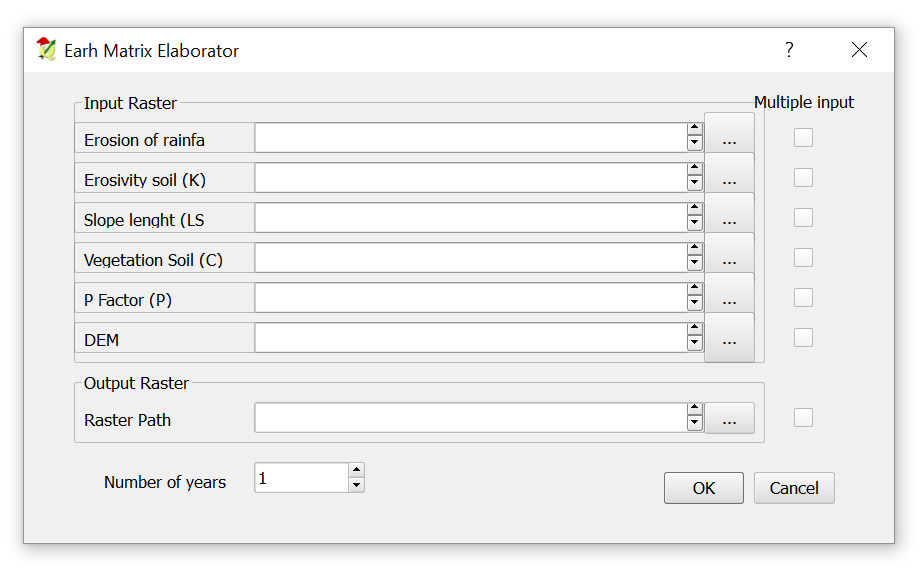
\includegraphics[width=\linewidth]{Capitoli/img/interfaccia.png}
	\caption{La finestre di configurazione dell'input e output del plugin. Permette di indicare il path dei file in modo grafico utilizzando la finestra standard di selezione del file del sistema operativo che si sta utilizzando.}
	\label{fig:screen1}
\end{figure}

\subsubsection{Qt4}

Le librerie grafiche per Python\footnote{Il linguaggio in cui è stato scritto il plugin} sono molte e varie ma la scelta è stata abbastanza facile: QT versione 4.

Questa scelta è stata dettata dal desiderio di ridurre al minimo le dipendenze esterne dal plugin. Questo comporta l'utilizzo preferenziale delle librerie utilizzate da QGis per semplificare l'installazione delle dipendenze. In particolare, con QGis è stato necessario scegliere anche la versione di QT con cui sviluppare il plugin in modo da non avere versioni differenti di QT rispetto a quella utilizzata QGis. La scelta è stata fatta su QT4 ovvero la funzione supportata dalla versione 2.0 in poi di QGis.  Questo permette la completa compatibilità di tutte le versioni esistenti supportate di QGis\footnote{Il plugin non è compatibile con QGis versioni antecedenti alla 2.x in quanto quelle versioni non sono più considerate stabili e non vengono più aggiornate. Questo perché quelle versioni utilizzano versioni precedenti di QT che porta ad renderizzare la grafica in modo corretto}.

La versione QT5 che verrà impiegata per le future versioni di QGis è già interamente supportata dal plugin. Questo è stato possibile attraverso un attento sviluppo attraverso funzioni non deprecate e controllo continuo delle nuove funzionalità di QT5 e delle modifiche che questa fa nel funzionamento complessivo in modo di essere già compatibile quando sarà necessario passare a QT5 in quanto QT4 non sarà più prerequisito di QGis venendo sostituito da QT5.

Ovviamente si poteva avere lo stesso risultato utilizzando altre librerie grafiche esterne o quelle di Python ma è stato scelto QT anche per avere una coerenza grafica tra le varie finestre che vanno ad aprirsi. Infatti se venisse utilizzata un altra libreria grafica sarebbe necessario una rielaborazione della grafica standard delle librerie in modo che si comportino coerentemente rispetto a QT e QGis per ogni sistema operativo, il che porterebbe a una complicazione del codice non necessaria\footnote{\egrave considerata non necessarie in quanto non porta vantaggi al sistema e ne aumenta la quantità rendendolo più complesso da mantenere}.

\subsection{Leggere e scrivere i dati}
Il plugin prende in ingresso i file contenenti i dati necessari per l'applicazione al modello matematico descritto dall'equazione \ref{eq:main}. Quindi, una volta eseguite le operazioni produce l'output corrispondente all'erosione per il numero di anni dati in input.

Le operazioni di lettura e scrittura sono le operazioni più sensibili in questo applictivo in quanto non c'è modo di controllare la correttezza dei dati in input dal punto di vista fisico/geologico, solo dal punto di vista informatico di buona formattazione.

\subsubsection{Input}
Per una questione di coerenza rispetto a QGis è stato deciso di passare i dati in input come file, in modo che possano essere facilmente condivisi e possano interagire più facilmente con QGis stesso. Per fare ciò è stato necessario fare una ricerca sui tipi di file utilizzati per i dati georefernziati.

Per questo motivo è stata fatta una ricerca sui formati di file supportati nativamente da QGis che fossero di tipo raster\footnote{Unico tipo di dati che il plugin accetta in input in quanto è l'unica struttura dati adatta a contenere i dati che ci servono per l'elaborazione} e quali fossero supportati attraverso plugin esterni.

E' stata quindi usata una delle funzioni del core di QGis per il riconoscimento automatico dei formati riconosciuti da QGis in modo da eseguire l'elaborazione del singolo file col driver corrispondente installato migliore.

Questo permette di avere un plugin più elastico, in quanto non necessita di aggiornamento se viene aggiunto il supporto a un tipo aggiuntivo di file per QGis ma recupera direttamente dalle configurazioni di QGis i dati necessari per la lettura, decodifica e rielaborazione del file in questione.

In oltre, il codice di gestione per i file in input è integrato nell'interfaccia grafica in modo da rendere semplice l'inserimento di dati all'interno del programma stesso. Supporta comunque l'utilizzo attraverso il terminale di QGis anche se ne è sconsigliato l'uso ai meno esperti e a chi si approccia per la prima volta a questo plugin.
%TODO inserire immagine apertura file

Come vedete dall'immagine il plugin apre una finestra di sistema differente in base al sistema operativo utilizzato, in quanto la gestione della scelta del file è delagato a esso. Una volta avvenuta la scelta questa finestra si chiuderà passando la stringa corrispondente al path del file aperto al campo adiacente presente nella gui principale. %TODO inserire riferimento a immagine gui generale
Se l'utente lo desidera puo' editare o direttamente inserire il path al file scelto direttamente nel campo senza aprire la finestra per la scelta della cartella.

Il file raster ricevuto in input viene quindi separato nelle sue componenti. Il file raster infatti è composto da due componenti:
\begin{itemize}
	\item una matrice che contiene i dati di interesse di quel raster
	\item una enupla legata ai dati della matrice
\end{itemize}
Questo meccanismo permette di avere dei dati che permettono di definire meglio i dati rappresentati nella matrice. Questi dati sono :

\begin{itemize}
	\item Numero di righe e colonne della matrice. Serve per avere la dimensione della matrice.
	\item Coordinate spaziali. Danno la posizione georeferenziata per la costruzione della matrice.
	\item Dimensioni della cella della matrice. Misura rappresentante la lunghezza e la larghezza dell'area di terreno i cui dati sono rappresentati dalla cella. Assieme alle coordinate spaziali serve a identificare l'area rappresentata dal file raster.
	\item Tipo di dato. Contiene delle informazioni rispetto al tipo di dato contenuto nelle celle. Questo è uniformo per tutto il file raster.
\end{itemize}

Questi dati non sono sempre presenti all'interno del file raster in quanto alcuni formati hanno per definizione uno di questi campi fissati a un valore, per cui sta al driver di qgis leggere i file in modo corretto e ritornare un enupla contenente i dati necessari.

Anche se presenti sempre non siamo interessati ai campi che specificano il software utilizzato per la creazione dei file, il copyright con cui vengono distribuiti e la data di creazione del file per cui non li leggiamo.

Una volta letti i dati di un raster vengono immagazzinati in una enupla, di più facile gestione, che viene elaborata dal plugin.

\subsubsection{Output}
Come per l'input, l'output può essere gestito in due modi: attraverso il terminale python o via interfaccia grafica.

In entrambi i casi è possibile indicare il path e il nome del file di output e il formato in cui lo si vuole salvare.
Il formato è scelto dall'utente da un elenco di formati disponibili nativamente da QGis con l'aggiunta dei formati disponibili da i plugin installati\footnote{Solo se questi registrano il formato nell'elenco nativamente presente in QGis come indicato dalle API per sviluppatori.} con driver per la scrittura. Per come è costruito QGis è possibile che alcuni formati non siano disponibili per la scrittura in quanto i driver sono di solo lettura. In questo caso, indipendentemente dalla scelta di utilizzare il terminale o una gui il plugin lancerà una finestra con l'errore corrispondente all'errore lanciato dal driver. Questo viene fatto in quanto è possibile che i formati in input non possono essere correttamente codificati nel formato di output scelto.

In ogni caso si consiglia che il formato di input e output dei file sia lo stesso per avere il minor problemi dati dalla decodifica e codifica degli stessi.

Nel casos i driver non vengono registrati all'interno dell'elenco dei driver per l'output di QGis seguendo le api sarà necessario implementarle sequendole per poterle utilizzare all'interno del plugin.

%TODO Spiegare la scrittura di raster
\subsection{Elaborazione dati}
Una volta ricevuti i dati in input si pensa a elaborarli. Per farlo è stato necessario generare una struttura dati idonea ai formati in input. E' stato quindi deciso di implementare l'elaborazione attraverso la struttura dati raster. A sua volta i dati geomorfici del raster sono all'interno di una matrice, che è l'oggetto con cui il plugin esegue le operazioni.

In oltre è stato necessario trovare una o più librerie che implementassero le funzionalità richieste per l'elaborazione dei dati raster mantenendo al minimo le dipendenze esterne. In caso di assenza di librerie si sarebbe dovuto implementare tutto da zero. Per nostra fortuna sono disponibili alcune librerie che eseguono calcoli in raster.

\subsubsection{Grass}
Plugin standard che da accesso a tutte le funzionalità avanzate di GRASS GIS. Dal punto di vista tecnico non è una libreria ma un insieme di librerie che gestiscono raster e elaborazioni avanzate dei dati. Essendo di facile installazione e, in alcune versioni, distribuito direttamente con QGis è un ottimo sistema per avere facilmente una libreria per l'elaborazione dei raster.

Il plugin descritto in questa tesi richiede l'istallazione di Grass per il suo corretto funzionamento anche se non usa direttamente la libreria di Grass.

La libreria di Grass non è stata usata direttamente ma solo una delle sue componenti per avere maggiore libertà nei formati disponibili di file. Infatti, a meno di un ridotto numero di plugin, non è possibile aumentare i tipi di file supportati da Grass in quanto si limitano solo ai formati forniti con l'installazione standard di QGis.

\subsubsection{Osgeo}
Una delle librerie utilizzate da Grass. Formalmente è una libreria per il supporto di operazioni su raster, in pratica è un porting di Numpy per i formati di file contenenti dati georeferenziati.

%TODO Spiegare in dettaglio cosa fa la libreria e come la utilizziamo
